\documentclass[12pt, twoside]{article}
\usepackage[letterpaper, margin=1in, headsep=0.5in]{geometry}
\usepackage[english]{babel}
\usepackage[utf8]{inputenc}
\usepackage{amsmath}
\usepackage{amsfonts}
\usepackage{amssymb}
\usepackage{tikz}
%\usetikzlibrary{quotes, angles}

\usepackage{graphicx}
\usepackage{enumitem}
\usepackage{multicol}

\usepackage{fancyhdr}
\pagestyle{fancy}
\fancyhf{}
\renewcommand{\headrulewidth}{0pt} % disable the underline of the header

\fancyhead[RE]{\thepage}
\fancyhead[RO]{\thepage \\ Name: \hspace{3cm}}
\fancyhead[L]{BECA / Dr. Huson / 10th Grade Geometry\\* Unit 7: Analytic Geometry Review\\15 February 2019}

\begin{document}
\subsubsection*{7-13 Break Packet: Linear \& quadratic functions on the coordinate plane}
  \begin{enumerate}

  \item Graph and label the two equations. Mark their intersection as an ordered pair.

    \begin{multicols}{2}
      $y = -4x-6$ \\
      $x-3y = -21$
    \end{multicols}  \vspace{1cm}
    Are the lines parallel, perpendicular, or neither? Justify your answer.
    \vspace{1.5cm}

    \begin{center} %4 quadrant regents grid w T-Chart
    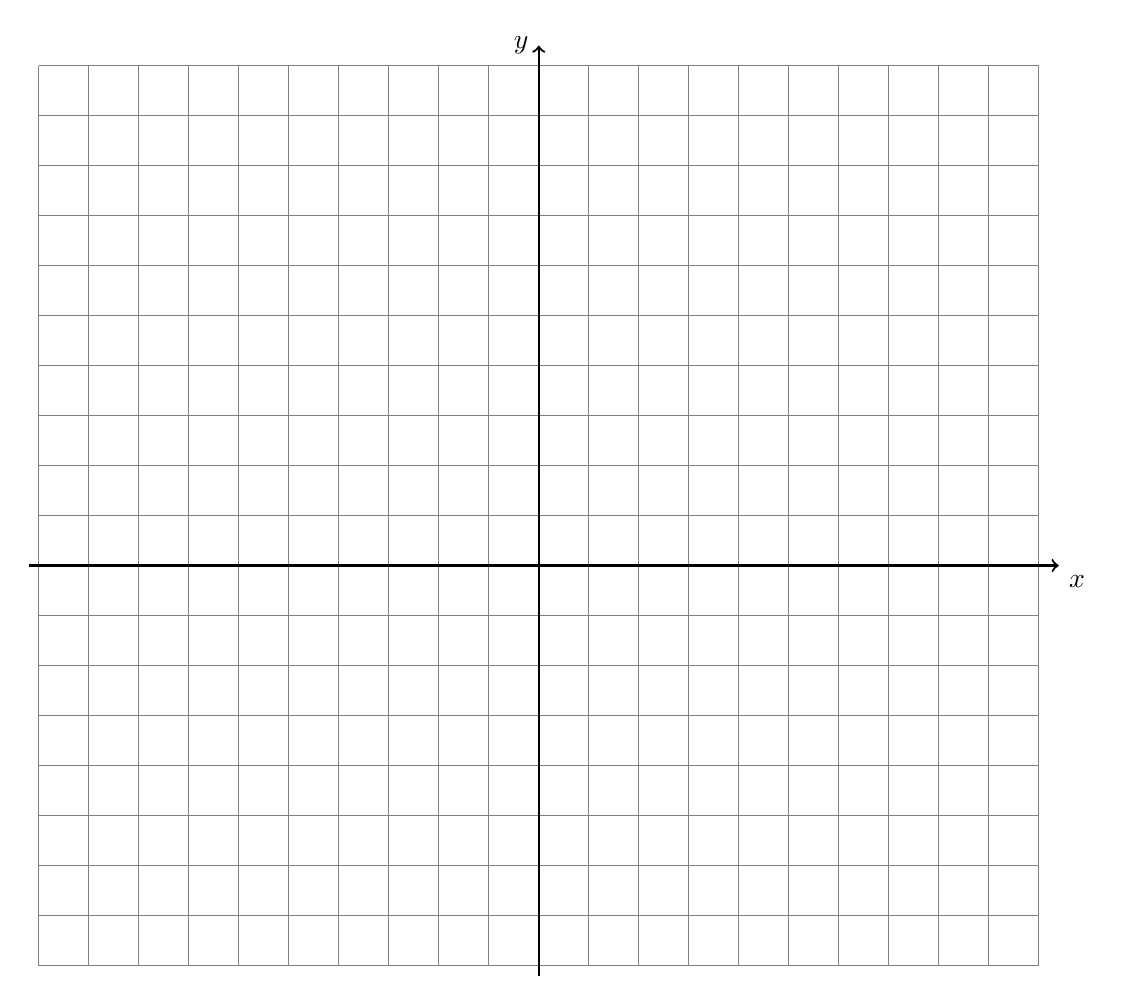
\begin{tikzpicture}[scale=.635]
      \draw [help lines] (-10,-8) grid (10,10);
      \draw [thick, ->] (-10.2,0) -- (10.4,0) node [below right] {$x$};
      \draw [thick, ->] (0,-8.2)--(0,10.4) node [left] {$y$};
    \end{tikzpicture}
    \end{center}

  \item The line $l$ has the equation $y= 3x+2$.
  \begin{enumerate}
    \item What is the slope of the line $k$, given $k \parallel l$?
    \vspace{1cm}
    \item What is the slope of the line $m$, given $m \perp l$?
    \vspace{1cm}
  \end{enumerate}

\newpage

  \item On the graph below, draw $\overline{AB}$, with $A(-1,1)$ and $B(7,3)$, labeling the end points. Determine and state the coordinates of the midpoint $M$ of $\overline{AB}$ and mark and label it on the graph.\\
    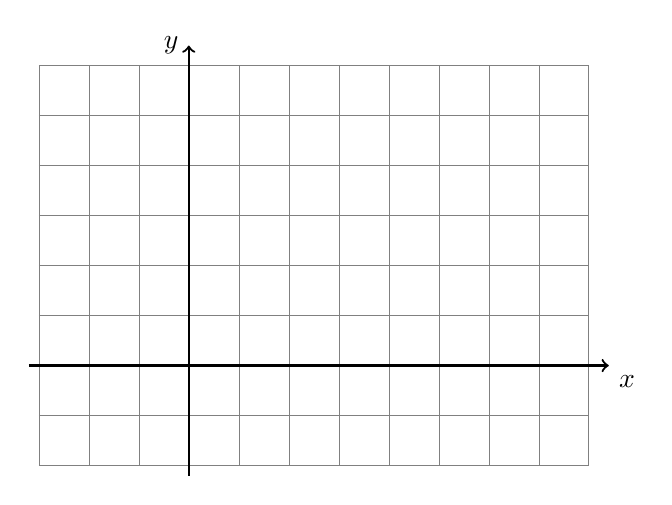
\begin{tikzpicture}[scale=.635]
      \draw [help lines] (-3,-2) grid (8,6);
      \draw [thick, ->] (-3.2,0) -- (8.4,0) node [below right] {$x$};
      \draw [thick, ->] (0,-2.2)--(0,6.4) node [left] {$y$};
    \end{tikzpicture}
    \vspace{1.5cm}

  \item Given $M(-1,0)$ and $N(3,-2)$, find the length of $\overline{MN}$. Simplify the radical.
      \vspace{5cm}

  \item $A(-1,7)$ is one endpoint of $\overline{AB}$. The segment's midpoint is $M(1,2)$. Find the other endpoint, $B$.

\newpage

  \item In the diagram below, $\overline{AC}$ has endpoints with coordinates $A(-6,-3)$ and $C(6, 3)$.
    \begin{center} %4 quadrant regents grid
      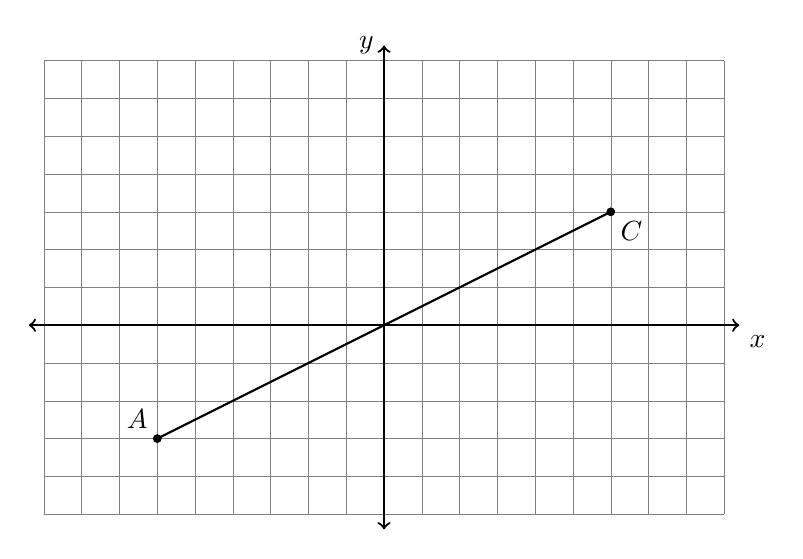
\begin{tikzpicture}[scale=.48]
        \draw [help lines] (-9,-5) grid (9,7);
        \draw [thick, <->] (-9.4,0) -- (9.4,0) node [below right] {$x$};
        \draw [thick, <->] (0,-5.4)--(0,7.4) node [left] {$y$};
        \draw [thick] (-6,-3)--(6, 3);
        \draw [fill] (-6,-3) circle [radius=0.1] node[above left] {$A$};
        \draw [fill] (6, 3) circle [radius=0.1] node[below right] {$C$};
      \end{tikzpicture}
    \end{center}
    If $B$ is a point on $\overline{AC}$ and $AB {:} BC = 1{:}3$,  what  are  the coordinates of $B$? \vspace{5cm}

  \item Write down the center and radius of each circle.
    \begin{enumerate}
      \begin{multicols}{2}
      \item   $(x-4)^2+(y-3)^2=9$ \vspace{2.5cm}
      \item   $(x+5)^2+(y-2)^2=4^2$
      \item   $x^2+y^2=4$ \vspace{2.5cm}
      \item   $(x+7)^2+(y-2)^2=9^2$
      \end{multicols}
    \end{enumerate}

\newpage

  In the following two problems, solve for the value of $x$.
  \begin{multicols}{2}
  \item   $\frac{1}{2}(3x+5)=7$ \vspace{4cm}
  \item   $\frac{2}{3}(6-12x)=-12$ \vspace{5cm}
  \end{multicols}

\vspace{4cm}

  \item Given $f(x)=\frac{1}{2} x+1$. Solve for $x$ such that for $f(x)=2$. \vspace{4cm}
  \item Given $g(x)=2x^2-7x+1$. Simplify $g(-1)$. \vspace{3cm}
  \item Given $h(x)=x^2-8x+16$. Solve $h(x)=0$. \vspace{3cm}

\newpage

  \item Complete the t-chart for $x=-5, -4, -3, -2, -1, 0$, then graph and label the function on the grid below. Use pencil for graphs. Draw parabolas as smooth curves.

      \[f(x) = (x+3)^2-4\]


    \begin{center} %4 quadrant regents grid w T-Chart
    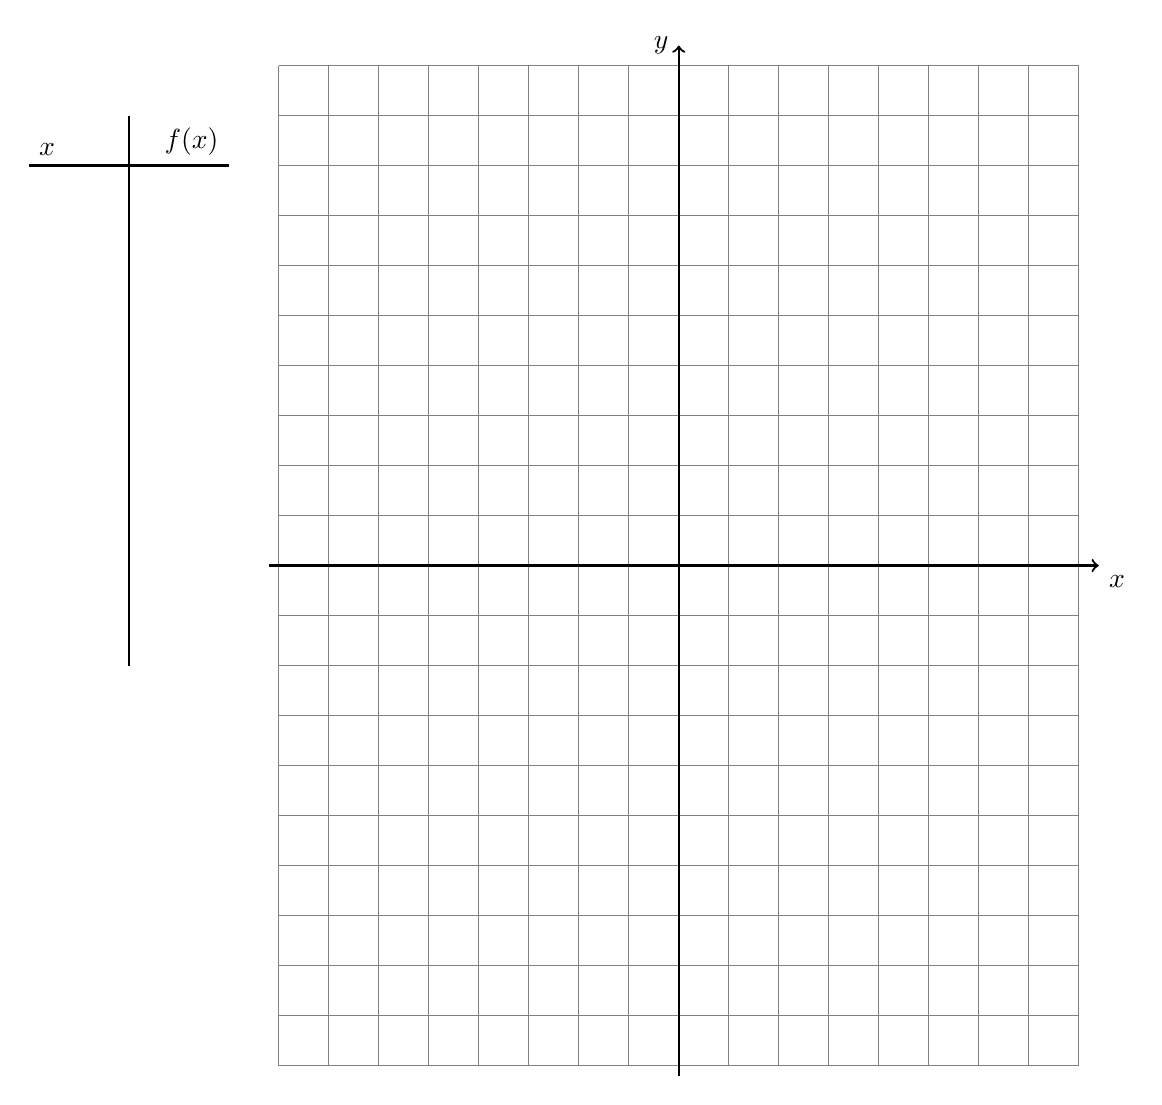
\begin{tikzpicture}[scale=.635]
      \draw [help lines] (-6,-10) grid (10,10);
      \draw [thick, ->] (-6.2,0) -- (10.4,0) node [below right] {$x$};
      \draw [thick, ->] (2,-10.2)--(2,10.4) node [left] {$y$};
      \draw [thick] (-11,8) node[above right]{$x$} --(-7,8) node [above left]{$f(x)$};
      \draw [thick] (-9,9)--(-9,-2);
    \end{tikzpicture}
    \end{center}

  \begin{enumerate}
    \item Mark the vertex on the graph as an ordered pair.
    \item Write down the equation for the axis of symmetry. \vspace{1.5cm}
    \item The function is translated four units to the right and three units up, $f \rightarrow g$. What is the equation of $g$?
  \end{enumerate}

  \newpage

  \item Spicy: On the set of axes below, graph the quadrilateral $ABCD$ having coordinates $A(-3,-3)$, $B(5,1)$, $C(6,8)$, and $D(-2,4)$.
    \begin{center} %4 quadrant regents grid
    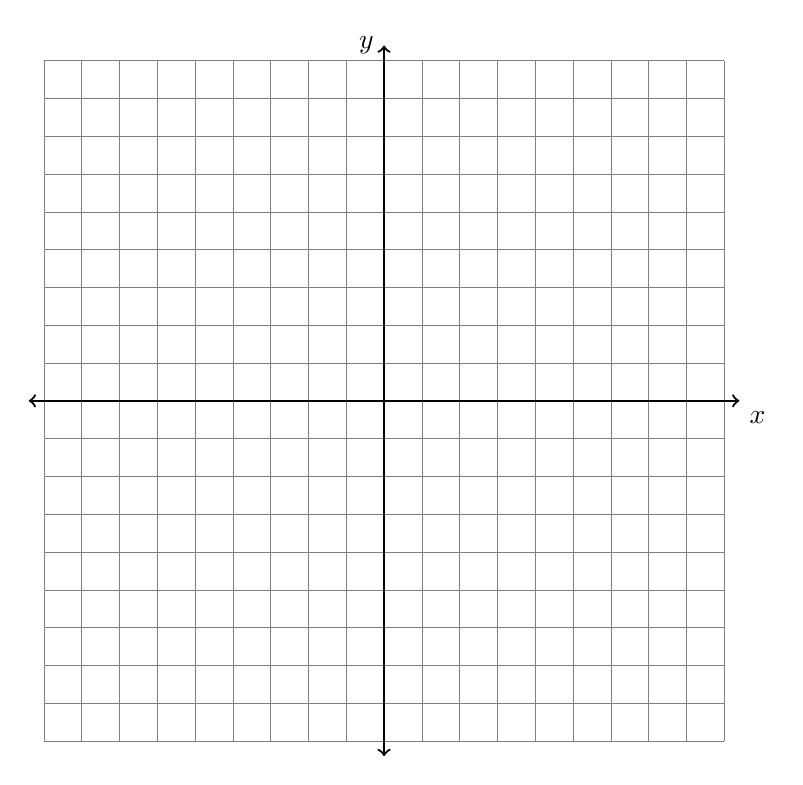
\begin{tikzpicture}[scale=.48]
      \draw [help lines] (-9,-9) grid (9,9);
      \draw [thick, <->] (-9.4,0) -- (9.4,0) node [below right] {$x$};
      \draw [thick, <->] (0,-9.4)--(0,9.4) node [left] {$y$};
      %\draw [thick] (-3,-3) node[below] {$A$}--
      %(5,1) node[right] {$B$}--
      %(6,8) node[left] {$C$}--
      %(-2,4) node[left] {$D$}--cycle;
      %\draw [fill] (5,0) circle [radius=0.1] node[above left] {$P$};
    \end{tikzpicture}
    \end{center}
    Show that the midpoints of the two diagonals, $\overline{AC}$ and $\overline{BD}$, are the same point. \\[5cm]
    Prove $ABCD$ is a parallelogram. Use the following theorem:
    A quadrilateral is a parallelogram if and only if its diagonals bisect each other. \\[0.5cm]
    Be sure to state the conclusion in your proof.



  \end{enumerate}

  \end{document}

  \newpage
  \newpage


    \item $\triangle ABC$ is shown with $m\angle C=90^\circ$. The lengths of the triangle's sides are $a$, $b$, and $c$. Express each trigonometric ratio as a fraction of two variables. \vspace{1cm}
    \begin{multicols}{2}
        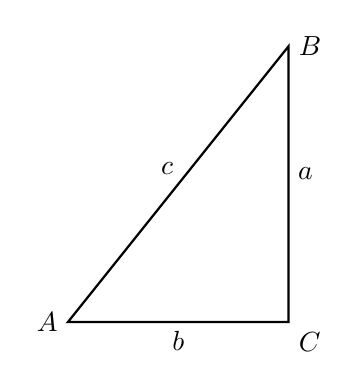
\begin{tikzpicture}[scale=0.7]
          \draw [thick]
          (0,0)node[left]{$A$}--
          (4,0)node[below right]{$C$}--
          (4,5)node[right]{$B$}--cycle;
          \node at (2,0)[below]{$b$};
          \node at (4,2.7)[right]{$a$};
          \node at (1.8,2.5)[above]{$c$};
        \end{tikzpicture}

          \begin{enumerate}
          \item $\sin B =$ \vspace{0.75cm}
          \item $\cos B =$ \vspace{0.75cm}
          \item $\tan B =$ \vspace{0.75cm}
        \end{enumerate}
    \end{multicols}

  \item Given two vertical angles, $m \angle 1 = 5x+9$, $m \angle 2 = 6x-1$. Find $m \angle 1$.\\
  For full credit, check by comparing to $m\angle 2$.
      \begin{flushright}
      \begin{tikzpicture}[scale=.7]
        \draw [<->, thick] (0,-1.5)--(10,1.5);
        \draw [<->, thick] (2,3.5)--(7,-3.5);
        \node at (3,.4){1};
        \node at (6,-.6){2};
      \end{tikzpicture}
      \end{flushright}

  \item Given $\overrightarrow{BA} \perp \overrightarrow{BC}$, $m \angle ABD = 10x+15$, and $m \angle DBC = 5x$. Find $m \angle DBC$. \\[0.5cm]
  For full credit, show the check using both angle measures.
    \begin{flushleft}
    \begin{tikzpicture}[scale=1.3]
      \draw [<->, thick] (0,3)--(0,0)--(5,0);
      \draw [->, thick] (0,0)--(3.5, 2);
      \draw [-, thin] (0, 0.4)--(0.4, 0.4)--(0.4, 0);
      %\node at (3,.4){1};
      %\node at (6,-.6){2};
      \draw [fill] (0,0) circle [radius=0.05] node[below]{$B$};
      \draw [fill] (0,2) circle [radius=0.05] node[left]{$A$};
      \draw [fill] (4,0) circle [radius=0.05] node[below]{$C$};
      \draw [fill] (2.625, 1.5) circle [radius=0.05] node[below]{$D$};
    \end{tikzpicture}
    \end{flushleft}
    \vspace{3cm}

    \item Given the circle $C$ with circumference $12\pi$.
  \begin{enumerate}
    \item Write down the formula for the circumference of a circle and solve for the radius yielding a circumference of $12\pi$. \vspace{1cm}
    \item Find the area of the circle.
  \end{enumerate}
  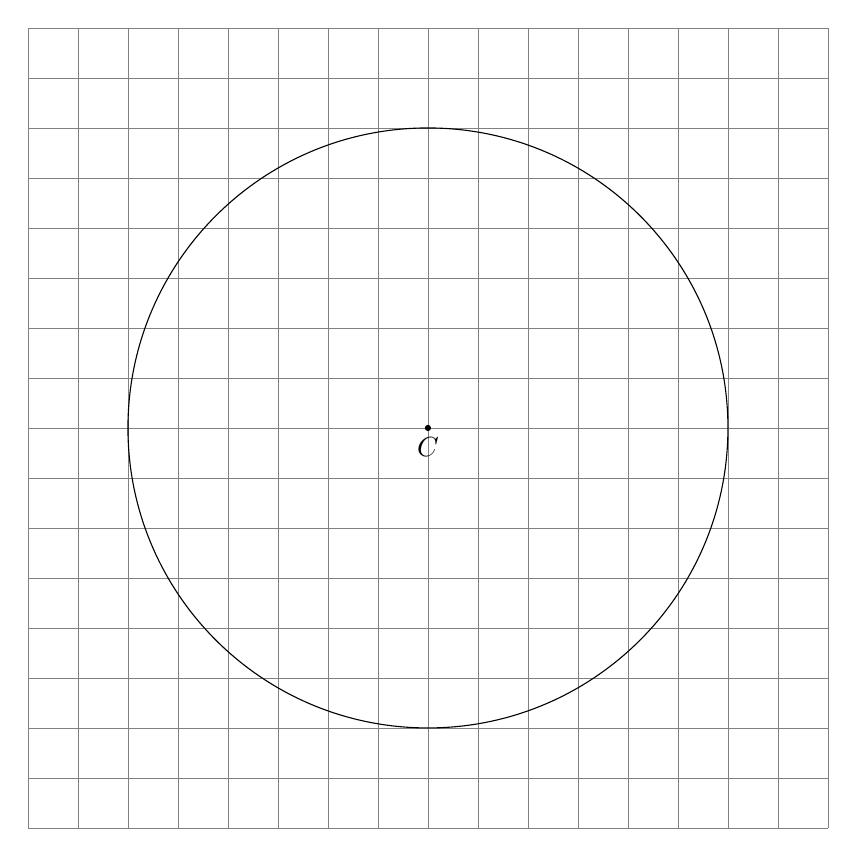
\begin{tikzpicture}[scale=.635]
    \draw [help lines] (-8,-8) grid (8,8);
    %\draw [thick, ->] (-2.2,0) -- (10.4,0) node [below right] {$x$};
    %\draw [thick, ->] (0,-2.2)--(0,10.4) node [left] {$y$};
    \draw (0,0) circle [radius=6] node[below]{$C$};
    \draw [fill] (0,0) circle [radius=0.05];
  \end{tikzpicture}

  \item On the graph, draw polygon ABCDEF with vertices A(1, 1), B(1, 4), C(3, 4), D(3, 7), E(8, 7), and F(8, 1). Find the perimeter and the area of the polygon.\\[1cm]
  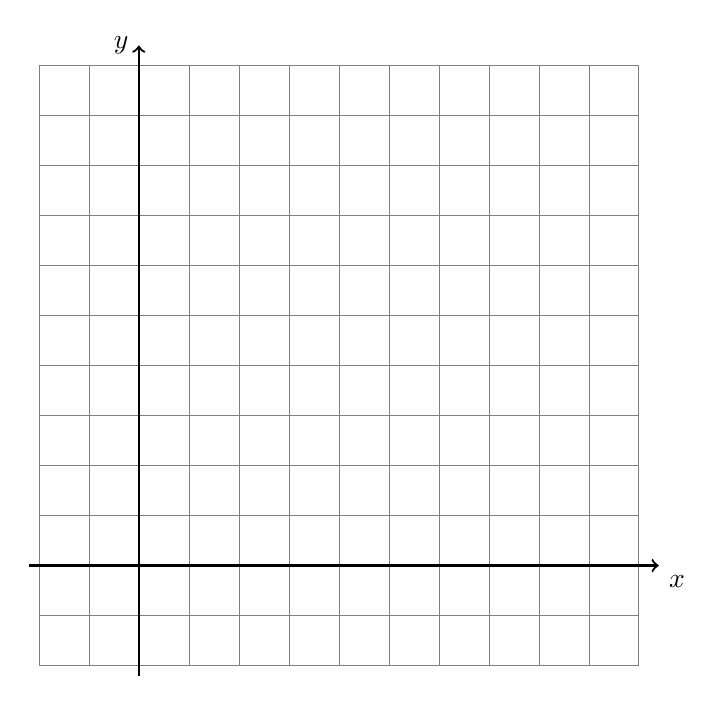
\begin{tikzpicture}[scale=.635]
    \draw [help lines] (-2,-2) grid (10,10);
    \draw [thick, ->] (-2.2,0) -- (10.4,0) node [below right] {$x$};
    \draw [thick, ->] (0,-2.2)--(0,10.4) node [left] {$y$};
  \end{tikzpicture}
  \vspace{2cm}

  \item Given a circle $O$ with radius $5$.
  \begin{enumerate}
    \item Find the circumference of $O$. \vspace{2cm}
    \item Find the area of $O$. \vspace{2cm}
  \end{enumerate}


\newpage

  \item Given $\overline{JKL}$, $JL=24$, and the point $K$ partitions $\overline{JL}$ in a ratio of 1:3.\\[0.5cm] Find ${JK}$. \\[1.5cm]
      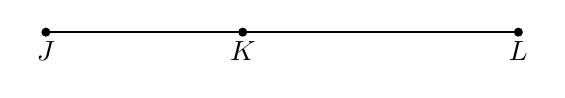
\begin{tikzpicture}
        \draw [-, thick] (1,0)--(7,0);
        \draw [fill] (1,0) circle [radius=0.05] node[below]{$J$};
        \draw [fill] (3.5,0) circle [radius=0.05] node[below]{$K$};
        \draw [fill] (7,0) circle [radius=0.05] node[below]{$L$};
      \end{tikzpicture} \vspace{3cm}
